%!TEX root = ceres.tex
\chapter{Tutorial}
\label{chapter:tutorial}

\section{Non-linear Least Squares}
\label{sec:tutorial:nonlinsq}
Let $x \in \reals^n$ be an $n$-dimensional vector of variables, and
$F(x) = \left[f_1(x); \hdots ; f_k(x)\right]$ be a vector of residuals $f_i(x)$. 
The function $f_i(x)$ can be a scalar or a vector valued
function.   We are interested in finding the solution to the following optimization problem
\begin{equation}
	\arg \min_x \frac{1}{2} \sum_{i=1}^k \|f_i(x)\|^2.
\end{equation}
Here $\|\cdot\|$ denotes the Euclidean norm of a vector. 

Such optimization problems arise in almost every area of science and engineering. Whenever there is data to be analyzed, curves to be fitted, there is usually a linear or a non-linear least squares problem lurking in there somewhere. 

Perhaps the simplest example of such a problem is the problem of Ordinary Linear Regression, where given observations $(x_1,y_1),\hdots, (x_k,y_k)$, we wish to find the line $y = mx + c$, that best explains $y$ as a function of $x$. One way to solve this problem is to find the solution to the following optimization problem
\begin{equation}
		\arg\min_{m,c} \sum_{i=1}^k (y_i - m x_i - c)^2
\end{equation}
With a little bit of calculus, this problem can be solved easily by hand. But what if, instead of a line we were interested in a more complicated relationship between $x$ and $y$, say for example $y = e^{mx + c}$. Then the optimization problem becomes
\begin{equation}
		\arg\min_{m,c} \sum_{i=1}^k \left(y_i - e^{m x_i + c}\right)^2
\end{equation}
This is a  non-linear regression problem and solving it by hand is much more tedious.  Ceres is designed to help you model and solve problems like this easily and efficiently.

\section{Hello World!}
\label{sec:tutorial:helloworld}
Let us consider the problem of finding the minimum of the function
\begin{equation}
	g(x) = \frac{1}{2}(10 -x)^2.
\end{equation}

This is a trivial problem, whose minimum is easy to see is located at 10, but it is a good place to start to illustrate the basics of solving a problem with Ceres. Let us write this problem as a non-linear least squares problem by defining the scalar residual function $f_1(x) = 10 - x$. Then $F(x) = [f_1(x)]$ is a residual vector with exactly one component.

When solving a problem with Ceres, the first thing to do is to define a \texttt{CostFunction}
object\footnote{Full working code for this and other examples in this manual can be found in the \texttt{examples} directory. Code for this example can be found in \texttt{examples/quadratic.cc}}. It is responsible for computing the value of the residual function and its derivative (also known as the Jacobian) with respect to $x$. Listing~\ref{listing:simplecostfunction} has the code.
\begin{listing}[H]
\begin{minted}[frame=lines]{c++}
class SimpleCostFunction
  : public ceres::SizedCostFunction<1 /* number of residuals */,
                                    1 /* size of first parameter */> {
 public:
  virtual ~SimpleCostFunction() {}
  virtual bool Evaluate(double const* const* parameters,
                        double* residuals,
                        double** jacobians) const {
    double x = parameters[0][0];
    // f(x) = 10 - x.
    residuals[0] = 10 - x;
    if (jacobians != NULL) {
	  // If the jacobians are asked for,
	  // then compute the derivative.
      jacobians[0][0] = -1;
    }
    return true;
  }
};
\end{minted}
\caption{A \texttt{CostFunction} for $f = 10 - x $}
\label{listing:simplecostfunction}
\end{listing}
\texttt{SimpleCostFunction} is provided with an input array of parameters, an output array for residuals and an optimal output array for Jacobians. In our example, there is just one parameter and one residual and this is known at compile time, therefore we inherit from templated \texttt{SizedCostFunction} class. The \texttt{jacobians} array is optional, \texttt{Evaluate} is expected to check when it is non-null, and if it is the case then fill it with the values of the derivative of the residual function. In this case since the residual function is linear, the Jacobian is constant.

Let us now look at the construction and solution of the problem using this \texttt{CostFunction}.
\begin{listing}[H]
\begin{minted}[frame=lines]{c++}
int main(int argc, char** argv) {
  double x = 5.0;
  ceres::Problem problem;

  // The problem object takes ownership of the newly allocated
  // SimpleCostFunction and uses it to optimize the value of x.
  problem.AddResidualBlock(new SimpleCostFunction, NULL, &x);

  // Configure the solver.
  ceres::Solver::Options options;
  options.max_num_iterations = 2;
  // Small, simple problem so we will use the Dense QR
  // factorization based solver.
  options.linear_solver_type = ceres::DENSE_QR;
  options.minimizer_progress_to_stdout = true;

  ceres::Solver::Summary summary;
  ceres::Solve(options, &problem, &summary);
  std::cout << summary.BriefSummary() << "\n";
  std::cout << "x : 5.0 -> " << x << "\n";
  return 0;
}
\end{minted}
\caption{Problem construction and solution for $F(x) = \frac{1}{2}(x-10)^2$}
\end{listing}

Compiling and running this program gives us
\begin{minted}{bash}
0: f: 1.250000e+01 d: 0.00e+00 g: 5.00e+00 h: 0.00e+00 rho: 0.00e+00 mu: 1.00e-04 li:  0
1: f: 1.249750e-07 d: 1.25e+01 g: 5.00e-04 h: 5.00e+00 rho: 1.00e+00 mu: 3.33e-05 li:  1
2: f: 1.388518e-16 d: 1.25e-07 g: 1.67e-08 h: 5.00e-04 rho: 1.00e+00 mu: 1.11e-05 li:  1
Ceres Solver Report: Iterations: 2, Initial cost: 1.250000e+01,  \
Final cost: 1.388518e-16, Termination: PARAMETER_TOLERANCE.
x : 5 -> 10
\end{minted}

Starting from a $x=5$, the solver in two iterations goes to 10. The careful reader will note that this is a linear problem and one linear solve should be enough to get the optimal value.  The default configuration of the solver is aimed at non-linear problems, and for reasons of simplicity we did not change it in this example. It is indeed possible to obtain the solution to this problem using Ceres in one iteration. Also note that the solver did get very close to the optimal function value of 0 in the very first iteration. We will discuss these issues in greater detail when we talk about convergence and initial parameter setting for Ceres.

\section{A Non-linear Example}
\label{sec:tutorial:powell}
Consider now a slightly more complicated example -- the minimization of Powell's function. Let $x = \left[x_1, x_2, x_3, x_4 \right]$ and
\begin{align}
   f_1(x) &= x_1 + 10*x_2 \\
   f_2(x) &= \sqrt{5} * (x_3 - x_4)\\
   f_3(x) &= (x_2 - 2*x_3)^2\\
   f_4(x) &= \sqrt{10} * (x_1 - x_4)^2\\
	F(x) & = \frac{1}{2}\left(f_1^2(x) + f_2^2(x) + f_3^2(x) + f_4^2(x) \right)
\end{align}
$F(x)$ is a function of four parameters, and has four residuals. Now,
one way to solve this problem would be to define four
\texttt{CostFunction}s that computes the residual and Jacobian. \eg Listing~\ref{listing:f4full} shows the implementation for $f_4(x)$.

\begin{listing}[H]
\begin{minted}[frame=lines,mathescape]{c++}
class F4 : public ceres::SizedCostFunction<1, 4> {
 public:
  virtual ~F4() {}
  virtual bool Evaluate(double const* const* parameters,
                        double* residuals,
                        double** jacobians) const {
    double x1 = parameters[0][0];
    double x4 = parameters[1][0];

    // $f_4 = \sqrt{10} * (x_1 - x_4)^2$
    residuals[0] = sqrt(10.0) * (x1 - x4) * (x1 - x4)
    if (jacobians != NULL) {
      // $\partial_{x_1}f_1(x)$
      jacobians[0][0] = 2.0 * sqrt(10.0) * (x1 - x4);
      // $\partial_{x_2}f_1(x)$
      jacobians[0][1] = 0.0;
      // $\partial_{x_3}f_1(x)$
      jacobians[0][2] = 0.0;
      // $\partial_{x_4}f_1(x)$
      jacobians[0][3] = -2.0 * sqrt(10.0) * (x1 - x4);
    }
    return true;
  }
};
\end{minted}
\caption{A full \texttt{CostFunction} implementation of $f_4(x) = \sqrt{10} * (x_1 - x_4)^2$.}
\label{listing:f4full}
\end{listing}

But this can get painful very quickly, especially for residuals involving complicated multivariate terms. Ceres provides two ways around this problem. Numeric and automatic symbolic differentiation.

\subsection{Automatic Differentiation}
\label{sec:tutorial:autodiff}
With its automatic differentiation support, Ceres allows you to define templated objects that will compute the residual and it takes care of computing the Jacobians as needed and filling the \texttt{jacobians} arrays with them.
For example, for $f_4(x)$ we define

\begin{listing}[H]
\begin{minted}[frame=lines,mathescape]{c++}
class F4 {
 public:
  template <typename T> bool operator()(const T* const x1,
                                        const T* const x4,
                                        T* residual) const {
    // $f_4 = \sqrt{10} * (x_1 - x_4)^2$
    residual[0] = T(sqrt(10.0)) * (x1[0] - x4[0]) * (x1[0] - x4[0]);
    return true;
  }
};
\end{minted}
\caption{Templated functor implementing $f_4(x) = \sqrt{10} * (x_1 - x_4)^2$ for use in automatic differentiation.}
\label{listing:f4functor}
\end{listing}

The important thing to note here is that the \texttt{operator()} is a
templated method, which assumes that all its inputs and outputs are of
some type \texttt{T}.  Note also that the parameters are not packed
into a single array, they are instead passed as separate arguments to
\texttt{operator()}. Similarly we can define classes \texttt{F1,F2}
and \texttt{F4}. Then let us consider the construction and solution of the problem. For brevity we only describe the relevant bits of code. The full source code for this example can be found in \texttt{examples/powell.cc}.

\begin{listing}[H]
\begin{minted}[frame=lines,mathescape]{c++}
double x1 =  3.0; double x2 = -1.0; double x3 =  0.0; double x4 =  1.0;

// Add residual terms to the problem using the using the autodiff
// wrapper to get the derivatives automatically. The parameters, x1 through
// x4, are modified in place.
problem.AddResidualBlock(
  new ceres::AutoDiffCostFunction<F1, 1, 1, 1>(new F1), NULL, &x1, &x2);
problem.AddResidualBlock(
  new ceres::AutoDiffCostFunction<F2, 1, 1, 1>(new F2), NULL, &x3, &x4);
problem.AddResidualBlock(
  new ceres::AutoDiffCostFunction<F3, 1, 1, 1>(new F3), NULL, &x2, &x3)
problem.AddResidualBlock(
  new ceres::AutoDiffCostFunction<F4, 1, 1, 1>(new F4), NULL, &x1, &x4);
\end{minted}
\caption{Problem construction using \texttt{AutoDiffCostFunction} for Powell's function.}
\label{listing:powell}
\end{listing}
A few things are worth noting in the code above. First, the object
being added to the \texttt{Problem} is an
\texttt{AutoDiffCostFunction} with \texttt{F1}, \texttt{F2}, \texttt{F3} and \texttt{F4} as template parameters. Second, each \texttt{ResidualBlock} only depends on the two parameters that the corresponding residual object depends on and not on all four parameters.


Compiling and running \texttt{powell.cc} gives us:
\begin{minted}{bash}
Initial x1 = 3, x2 = -1, x3 = 0, x4 = 1
   0: f: 1.075000e+02 d: 0.00e+00 g: 1.55e+02 h: 0.00e+00 rho: 0.00e+00 mu: 1.00e-04 li:  0
   1: f: 5.036190e+00 d: 1.02e+02 g: 2.00e+01 h: 2.16e+00 rho: 9.53e-01 mu: 3.33e-05 li:  1
   2: f: 3.148168e-01 d: 4.72e+00 g: 2.50e+00 h: 6.23e-01 rho: 9.37e-01 mu: 1.11e-05 li:  1
   3: f: 1.967760e-02 d: 2.95e-01 g: 3.13e-01 h: 3.08e-01 rho: 9.37e-01 mu: 3.70e-06 li:  1
   4: f: 1.229900e-03 d: 1.84e-02 g: 3.91e-02 h: 1.54e-01 rho: 9.37e-01 mu: 1.23e-06 li:  1
   5: f: 7.687123e-05 d: 1.15e-03 g: 4.89e-03 h: 7.69e-02 rho: 9.37e-01 mu: 4.12e-07 li:  1
   6: f: 4.804625e-06 d: 7.21e-05 g: 6.11e-04 h: 3.85e-02 rho: 9.37e-01 mu: 1.37e-07 li:  1
   7: f: 3.003028e-07 d: 4.50e-06 g: 7.64e-05 h: 1.92e-02 rho: 9.37e-01 mu: 4.57e-08 li:  1
   8: f: 1.877006e-08 d: 2.82e-07 g: 9.54e-06 h: 9.62e-03 rho: 9.37e-01 mu: 1.52e-08 li:  1
   9: f: 1.173223e-09 d: 1.76e-08 g: 1.19e-06 h: 4.81e-03 rho: 9.37e-01 mu: 5.08e-09 li:  1
  10: f: 7.333425e-11 d: 1.10e-09 g: 1.49e-07 h: 2.40e-03 rho: 9.37e-01 mu: 1.69e-09 li:  1
  11: f: 4.584044e-12 d: 6.88e-11 g: 1.86e-08 h: 1.20e-03 rho: 9.37e-01 mu: 5.65e-10 li:  1
Ceres Solver Report: Iterations: 12, Initial cost: 1.075000e+02, \
Final cost: 2.865573e-13, Termination: GRADIENT_TOLERANCE.
Final x1 = 0.000583994, x2 = -5.83994e-05, x3 = 9.55401e-05, x4 = 9.55401e-05
\end{minted}
It is easy to see that the  optimal solution to this problem is at $x_1=0, x_2=0, x_3=0, x_4=0$ with an objective function value of $0$. In 10 iterations, Ceres finds a solution with an objective function value of $4\times 10^{-12}$.

If a templated implementation is not possible then a \texttt{NumericDiffCostFunction} object can be used. \texttt{examples/quadratic\_numeric\_diff.cc} shows a numerically differentiated implementation of \texttt{examples/quadratic.cc}.

When possible, automatic differentiation should be used. The use of
C++ templates makes automatic differentiation extremely efficient,
whereas numeric differentiation can be quite expensive, prone to
numeric errors and leads to slower convergence.

\section{Data Fitting}
\label{sec:tutorial:datafitting}
The examples we have seen until now are simple optimization problems with no data. The original purpose of least squares and non-linear least squares analysis was fitting curves to data. It is only appropriate that we now consider an example of such a problem. Let us fit some data to the curve
\begin{equation}
	y = e^{mx + c}
\end{equation}

The full code and data for this example can be found in
\texttt{examples/data\_fitting.cc}. It contains data generated by sampling the curve $y = e^{0.3x + 0.1}$ and adding Gaussian noise with standard deviation $\sigma = 0.2$.

We begin by defining a templated object to evaluate the residual. There will be a residual for each observation.

\begin{listing}[H]
\begin{minted}[frame=lines,mathescape]{c++}
class ExponentialResidual {
 public:
  ExponentialResidual(double x, double y)
      : x_(x), y_(y) {}

  template <typename T> bool operator()(const T* const m,
                                        const T* const c,
                                        T* residual) const {
    // $y - e^{mx + c}$
    residual[0] = T(y_) - exp(m[0] * T(x_) + c[0]);
    return true;
  }

 private:
  // Observations for a sample.
  const double x_;
  const double y_;
};
\end{minted}
\caption{Templated functor to compute the residual for the exponential model fitting problem. Note that one instance of the functor is responsible for computing the residual for one observation.}
\label{listing:exponentialresidual}
\end{listing}
Assuming the observations are in a $2n$ sized array called \text{data}, the problem construction is a simple matter of creating a \texttt{CostFunction} for every observation.
\begin{listing}[H]
\begin{minted}[frame=lines,mathescape]{c++}
double m = 0.0;
double c = 0.0;

Problem problem;
for (int i = 0; i < kNumObservations; ++i) {
  problem.AddResidualBlock(
      new AutoDiffCostFunction<ExponentialResidual, 1, 1, 1>(
          new ExponentialResidual(data[2 * i], data[2 * i + 1])),
      NULL,
      &m, &c);
}
\end{minted}
\caption{Problem construction for the exponential data fitting problem. A \texttt{ResidualBlock} is added for each observation.}
\label{listing:datafitting}
\end{listing}
Compiling and running \texttt{data\_fitting.cc} gives us
\begin{minted}{bash}
 0: f: 1.211734e+02 d: 0.00e+00 g: 3.61e+02 h: 0.00e+00 rho: 0.00e+00 mu: 1.00e-04 li:  0
 1: f: 1.211734e+02 d:-2.21e+03 g: 3.61e+02 h: 7.52e-01 rho:-1.87e+01 mu: 2.00e-04 li:  1
 2: f: 1.211734e+02 d:-2.21e+03 g: 3.61e+02 h: 7.51e-01 rho:-1.86e+01 mu: 8.00e-04 li:  1
 3: f: 1.211734e+02 d:-2.19e+03 g: 3.61e+02 h: 7.48e-01 rho:-1.85e+01 mu: 6.40e-03 li:  1
 4: f: 1.211734e+02 d:-2.02e+03 g: 3.61e+02 h: 7.22e-01 rho:-1.70e+01 mu: 1.02e-01 li:  1
 5: f: 1.211734e+02 d:-7.34e+02 g: 3.61e+02 h: 5.78e-01 rho:-6.32e+00 mu: 3.28e+00 li:  1
 6: f: 3.306595e+01 d: 8.81e+01 g: 4.10e+02 h: 3.18e-01 rho: 1.37e+00 mu: 1.09e+00 li:  1
 7: f: 6.426770e+00 d: 2.66e+01 g: 1.81e+02 h: 1.29e-01 rho: 1.10e+00 mu: 3.64e-01 li:  1
 8: f: 3.344546e+00 d: 3.08e+00 g: 5.51e+01 h: 3.05e-02 rho: 1.03e+00 mu: 1.21e-01 li:  1
 9: f: 1.987485e+00 d: 1.36e+00 g: 2.33e+01 h: 8.87e-02 rho: 9.94e-01 mu: 4.05e-02 li:  1
10: f: 1.211585e+00 d: 7.76e-01 g: 8.22e+00 h: 1.05e-01 rho: 9.89e-01 mu: 1.35e-02 li:  1
11: f: 1.063265e+00 d: 1.48e-01 g: 1.44e+00 h: 6.06e-02 rho: 9.97e-01 mu: 4.49e-03 li:  1
12: f: 1.056795e+00 d: 6.47e-03 g: 1.18e-01 h: 1.47e-02 rho: 1.00e+00 mu: 1.50e-03 li:  1
13: f: 1.056751e+00 d: 4.39e-05 g: 3.79e-03 h: 1.28e-03 rho: 1.00e+00 mu: 4.99e-04 li:  1
Ceres Solver Report: Iterations: 13, Initial cost: 1.211734e+02, \
Final cost: 1.056751e+00, Termination: FUNCTION_TOLERANCE.
Initial m: 0 c: 0
Final   m: 0.291861 c: 0.131439
\end{minted}

\begin{figure}[t]
	\begin{center}
	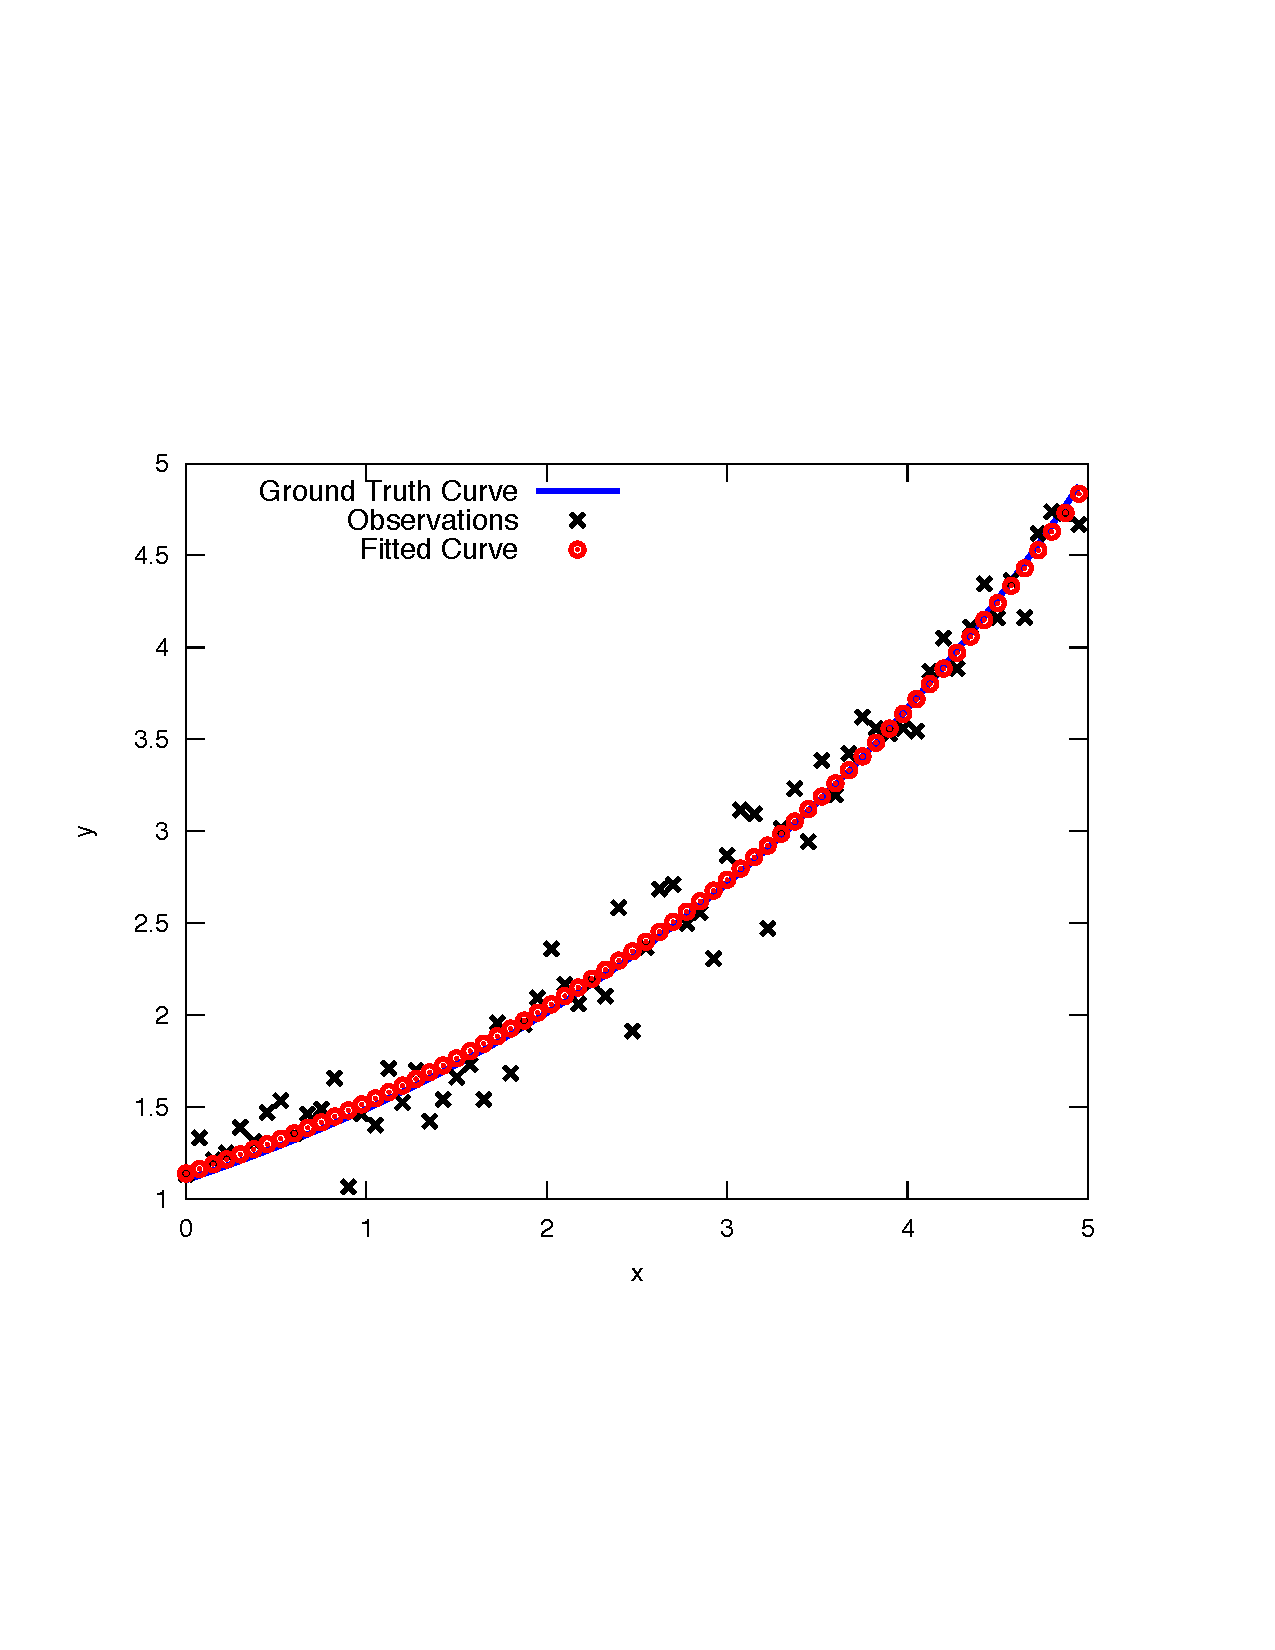
\includegraphics[width=\textwidth]{fit.pdf}
	\caption{Least squares data fitting to the curve $y = e^{0.3x + 0.1}$. Observations were generated by sampling this curve uniformly in the interval $x=(0,5)$ and adding Gaussian noise with $\sigma = 0.2$.\label{fig:exponential}}
\end{center}
\end{figure}

Starting from parameter values $m = 0, c=0$ with an initial objective function value of $121.173$ Ceres finds a solution $m= 0.291861, c = 0.131439$ with an objective function value of $1.05675$. These values are a a bit different than the parameters of the original model $m=0.3, c= 0.1$, but this is normal. When reconstructing a curve from noisy data, we expect to see such deviations. Indeed, if you were to evaluate the objective function for $m=0.3, c=0.1$, the fit is worse with an objective function value of 1.082425. Figure~\ref{fig:exponential} illustrates the fit.

\section{Bundle Adjustment}
\label{sec:tutorial:bundleadjustment}
\begin{listing}[ht]
\begin{minted}[frame=lines,mathescape]{c++}
struct SnavelyReprojectionError {
  SnavelyReprojectionError(double observed_x, double observed_y)
      : observed_x(observed_x), observed_y(observed_y) {}

  template <typename T>
  bool operator()(const T* const camera,
                  const T* const point,
                  T* residuals) const {
    // camera[0,1,2] are the angle-axis rotation.
    T p[3];
    ceres::AngleAxisRotatePoint(camera, point, p);
    // camera[3,4,5] are the translation.
    p[0] += camera[3]; p[1] += camera[4]; p[2] += camera[5];

    // Compute the center of distortion. The sign change comes from
    // the camera model that Noah Snavely's Bundler assumes, whereby
    // the camera coordinate system has a negative z axis.
    const T& focal = camera[6];
    T xp = - focal * p[0] / p[2];
    T yp = - focal * p[1] / p[2];

    // Apply second and fourth order radial distortion.
    const T& l1 = camera[7];
    const T& l2 = camera[8];
    T r2 = xp*xp + yp*yp;
    T distortion = T(1.0) + r2  * (l1 + l2  * r2);

    // Compute final projected point position.
    T predicted_x = distortion * xp;
    T predicted_y = distortion * yp;

    // The error is the difference between the predicted and observed position.
    residuals[0] = predicted_x - T(observed_x);
    residuals[1] = predicted_y - T(observed_y);
    return true;
  }

  double observed_x;
  double observed_y;
};
\end{minted}
\caption{Templated functor to compute the residual using the Bundler camera. Note that the structure of this functor is similar to the \texttt{ExponentialResidual}~\ref{listing:exponentialresidual}, in that there is an instance of this object responsible for each image observation. The camera has nine parameters. Three for rotation as a Rodriquez axis-angle vector, three for translation, one for focal length and two for radial distortion. \texttt{AngleAxisRotatePoint} can be found in \texttt{rotation.h}.}
\label{listing:bundlerresidual}
\end{listing}

One of the main reasons for writing Ceres was our desire to solve large scale bundle adjustment problems~\cite{hartley-zisserman-book-2004,triggs-etal-1999}.



Given a set of measured image feature locations and correspondences, the goal of bundle adjustment is to find 3D point positions and camera parameters that minimize the reprojection error. This optimization problem is usually formulated as a non-linear least squares problem, where the error is the squared $L_2$ norm of the difference between the observed feature location and the projection of the corresponding 3D point on the image plane of the camera.

Ceres has extensive support for solving bundle adjustment problems. Let us consider the solution of a problem from the BAL~\cite{Agarwal10bal} dataset. The code for this example can be found in \texttt{examples/simple\_bundle\_adjuster.cc}.

The first step is to define the CostFunction. Each residual in a BAL
problem depends on a three dimensional point and a nine parameter
camera. The details of this camera model can be found on Noah
Snavely's Bundler
homepage~\footnote{\url{http://phototour.cs.washington.edu/bundler/}}
and the BAL
homepage~\footnote{\url{http://grail.cs.washington.edu/projects/bal/}}. Listing~\ref{listing:bundlerresidual}
describes the templated functor for computing the residual. Unlike the
examples before this is a non-trivial function and computing its
analytic Jacobian is a bit of a pain. Automatic differentiation makes
our life very simple here. Given this functor, let us look at the problem construction.

\begin{minted}[frame=lines,mathescape]{c++}
// Create residuals for each observation in the bundle adjustment problem. The
// parameters for cameras and points are added automatically.
ceres::Problem problem;
for (int i = 0; i < bal_problem.num_observations(); ++i) {
  // Each Residual block takes a point and a camera as input and outputs a 2
  // dimensional residual. Internally, the cost function stores the observed
  // image location and compares the reprojection against the observation.
  ceres::CostFunction* cost_function =
      new ceres::AutoDiffCostFunction<SnavelyReprojectionError, 2, 9, 3>(
          new SnavelyReprojectionError(
              bal_problem.observations()[2 * i + 0],
              bal_problem.observations()[2 * i + 1]));

  problem.AddResidualBlock(cost_function,
                           NULL /* squared loss */,
                           bal_problem.mutable_camera_for_observation(i),
                           bal_problem.mutable_point_for_observation(i));
  }
}
\end{minted}

Note that the problem construction for bundle adjustment is not very
different from the data fitting example. One extra feature here is the
optional use of a robust loss function. If the user wants, instead of just using a squared reprojection error as the objective function we robustify it using Huber's loss. More details of the various loss functions available in Ceres and their characteristics can be found in \texttt{loss\_function.h}.

One way to solve this problem would be to set \texttt{Solver::Options::linear\_solver\_type} to \texttt{SPARSE\_NORMAL\_CHOLESKY} and call \texttt{Solve}. And while this is a reasonable thing to do, bundle adjustment problems have a special sparsity structure that can be exploited to solve them much more efficiently. Ceres provides three specialized solvers (collectively known as Schur based solvers) for this task. The example code uses the simplest of them \texttt{DENSE\_SCHUR}. For more details on the available solvers and how they work see Chapter~\ref{chapter:theory}.

For a more sophisticated example of bundle adjustment which demonstrates the use of the various linear solvers, robust loss functions and local parameterizations see \texttt{examples/bundle\_adjuster.cc}.